\capitolo{Dimensionamento e Scelta di Viti a Ricircolo di Sfere}
I riduttori vite madrevite classici sono a strisciamento e questa caratteristica li rende particolarmente soggetti all'attrito, quindi a ridotto rendimento e irreversibilità del moto. Queste sono caratteristiche desiderabili per strutture, meno per organi in moto, si fa largo la necessità di rendimenti superiori, quindi vengono utilizzate tecnologie differenti.

La principale delle tecnologie alternative è quella di riduttori a vite a ricircolo di sfere in cui lo spostamento viene trasmesso dalle sfere che rotolando permettono di avere ridotto attrito, quindi rendimento maggiore, indicativamente \( \eta_{R\rightarrow T} \simeq 0.97 \simeq \eta_{T\rightarrow R} \).

Le sfere sono poste all'interno di gole su cui possono scorrere, presenti al posto dei denti nella vite e madrevite, chiamata in questo contesto chiocciola.

\paragrafo{Configurazioni cinematiche:}
In termmini di cinematica le viti a ricircolo di sfere sono equivalenti alle viti-madreviti a strisciamento, in particolare vale ancora \( \tau_v = \frac{p}{2\pi} = \frac{\Delta x_{rel}}{\Delta \theta_{rel}} \), dove gli spostamenti sono considerati relativi.
In seguito sono rappresentate le varie combinazioni di movimenti assoluti.

\begin{figure}[h]
    \centering
    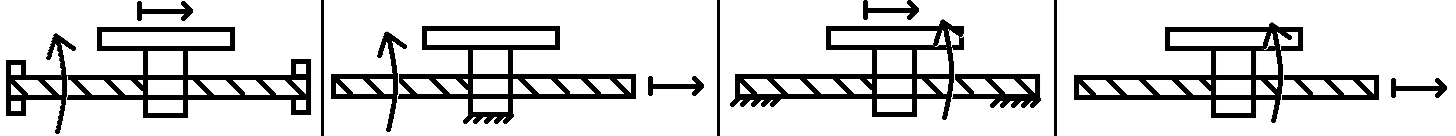
\includegraphics[width=0.9\textwidth]{Immagini/confi_din_vite_ricircolo.png}
    \caption{4 possibili configurazioni rotazione-traslazione relative}
\end{figure}

\sezione{Parametri di scelta}
La scelta di viti a ricircolo di sfere non è banale perché ha dipendenza da un alto numero di combinazioni possibili di diametri viti e sfere, passo della vite, vita utile, numero di principi e tipologia di materiali.

\paragrafo{Numero di principi:}
Con numero di principi si intendono i singoli percorsi indipendenti di ricircolo delle sfere. All'interno di un passo della vite potrebbe esserci sufficiente spazio per inserire un ulteriore ricircolo di sfere, così nasce una vite a due principi.

\sottosezione{Dinamica}
Similmente a come visto per i riduttori si vanno a definire la forza applicata sul carico: \( C_m = \left( J_m + J_v + M \frac{\tau_v^2}{\eta_v} \right) \AccAng_m + F \frac{\tau_v}{\eta_v} \), da cui, a seguito di opportuna manipolazione, si ottiene: \( C_m = \left(J_m + J_v\right) \frac{\Ddot x}{\tau_v} + \frac{\tau_v}{\eta_v} \left( M\Ddot x + F \right) \), dove:
\[ F_a = M\Ddot x + F \]
risultante delle forze assiali applicate alla chiocciola (equivalente a \( T_2 \) dei riduttori).

\begin{figure}[h]
    \centering
    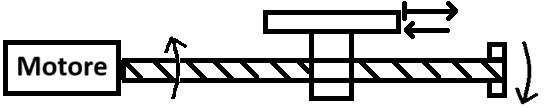
\includegraphics[width=0.4\textwidth]{Immagini/mot_vite_ricircolo.png}
    \caption{Schema motore e vite a ricircolo di sfere}
\end{figure}

\sottosottosezione{Forza assiale media}
Anche in questo caso nel regime stazionario si fanno valutazioni sulla media, e in modo simile a \( T_{2,media} \) si ottiene:
\[ F_{a, media} = \sqrt[3]{\frac{\int^{T_{ciclo}}_0 \abs{F_a^3(t)\Ddot{x}_c(t)dt}}{\int^{T_{ciclo}}_0 \abs{\Ddot{x}_c(t)}dt}} \]
E anche in questo caso per moto ad andamento trapezoidale l'integrale diventerà una sommatoria.

\sottosottosezione{Capacità di Carico Dinamico}
Per capacità di carico dinamico \( C_D [N] \) si intende nei cataloghi la forza assiale applicata alla  chiocciola che garantisce con probabilità di sopravvivenza del \(90\%\) la vita utile di \(10^6\) giri relativi vite-chiocciola.

\paragrafo{Migliorare la probabilità:}
Per migliorare la probabilità occorre utilizzare un fattore di affidabilità \(<1\) che vada a penalizzare il valore a catalogo. Si tratta di valori ricavati statisticamente, non hanno significato di coefficiente di sicurezza.

\paragrafo{Utilizzo di CCD in verifica:}
Noti \(C_D, F_{a, media}\), volendo calcolare la vita utile della chiocciola per il \(90\%\) di probabilità di sopravvivenza si utilizza la formula di Wohler: \( C_D^3 10^6 = F_{a,media}^3 L_N \), con \(L_N\) vita utile in termini di numero di rotazioni.

\paragrafo{Utilizzo di CCD in dimensionamento:}
Noto \(F_{a,media}\), data dalla specifica in termini di giri sulla vita utile \(L_N^{des}\) desiderata, è possibile calcolare \(C_D\) idoneo a garantire la vita desiderata al \(x\%\) invertendo la formula e utilizzando un opportuno fattore di affidabilità.

\paragrafo{Vita utile in ore:}
Solitamente non è nota la vita utile in numero di giri relativi, è più comodo passare in ore di lavoro, quindi 
\[ L_H = L_N \frac{1}{\VelAng_v} \frac{1}{60} [h] = L_N \frac{p}{3600 \cdot \dot{x}_{media}} \]
che si traduce in una CCD richiesta: 
\[ C_{D,rich} \geqslant F_{a,media} \sqrt[3]{\frac{L_H^{des}\dot{x}^{des} \cdot 3600}{p \cdot 10^6}} f_s \]

\sottoparagrafo{Fattore di Shock/Servizio:}
Alla CCD in esame va moltiplicato un fattore di shock o servizio \( f_s \), i cui valori possono cambiare tra \( 1.2 \div 3 \), se possibile conviene utilizzare un modello elasto-dinamico per avere una idea delle forze in gioco e evitare di sovradimensionare la chiocciola.

\paragrafo{Dipendenze della CCD richiesta:}
La CCD è dipendente direttamente da velocità traslante e vita utile, mentre è inversamente dipendente dal passo \( p \downarrow, C_D \uparrow\). La dipendenza inversa del passo risulta chiara immaginando che i passi minori portano a un maggior numero di giri relativi a pari velocità.

\paragrafo{Dipendenze della CCD:}
Il carico dinamico sulla chiocciola dipende principalmente dal volume delle sfere e dal materiale delle stesse.
Come regola generale conviene avere meno sfere più grandi che tenderanno a raggiungere un volume complessivo maggiore, inoltre garantiscono una maggior resistenza.

%% inserire immagini pag 19 bassa, 20 alta

\sottosottosezione{Velocità limite delle sfere}
Durante il moto le sfere ruotano tra le due gole di vite e chiocciola, ma in questo movimento vanno anche a strisciare tra loro. Per velocità elevate risulta un aumento di riscaldamento e un aumento usura legato alla formazione di particolato di sfere.
La relazione da verificare è \( v_{sfere} = \VelAng_v \frac{d}{2} < v_{lim} \) dove \(d\) è la distanza tra centri delle due sfere opposte, e con velocità limite specifica della chiocciola.

Nei cataloghi non si tiene conto della velocità della sfera, ma del doppio, e viene chiamata "D \(\times\) n" \(= \VelAng_v\cdot d \), quindi  il limite diventa: \(d\VelAng_v < \text{"D}\times \text{n"}_{lim} \alpha = S \).  